Este capítulo detalha o \textit{BFT-SMaRt} apresentando seu conceito, princípios de projeto, protocolos centrais, reconfiguração, implementação, configurações alternativas e finalizando nas conclusões do capítulo.


%	\section{BTF-SMART}
	\section{Conceitos}
	Na área da computação, a replicação de máquina de estado (SMR) é um método para implementação de um serviço tolerante a falha, onde um conjunto de servidores trabalham coordenadamente para prover determinado serviço para a(s) máquina(s) cliente(s). \\
		
	O \textit{BFT-SMaRt} é uma biblioteca de código aberto criada recentemente em linguagem Java. É composta por um conjunto de classes capaz de implementar um sistema distribuído robusto consistindo pela replicação das máquinas de estado tolerantes a falhas bizantinas. Falha bizantina ocorre quando uma máquina apresenta um comportamento arbitrário fora de sua especificação, por exemplo, quando um servidor é invadido e começa a rodar código malicioso. Além disso, o \textit{BFT-SMaRt} apresenta confiabilidade, modularidade, reconhecimento de sistema \textit{multicore}, suporte à reconfiguração e interface flexível de programação, como foi apresentado por Alchieri et al em \cite{bessani3}. \\
	
	Novamente em \cite{bessani3} é abordado como nos últimos anos a discussão sobre replicação de máquina de estado (\textit{State Machine Replication - SMR}) tolerantes a falhas bizantinas (\textit{Byzantine Fault-Tolerant - BFT}) tem se acirrado contendo pouco avanço prático, apenas protótipos usados para validar ideias apresentadas em artigos, assim dificultando a aplicação dessa prática em aplicações reais. Os autores acreditam que isto seja devido à falta de implementações de um SMR BFT robusto. O \textit{BFT-SMaRt} foi proposto tendo em mente contornar tal dificuldade, o qual almeja tanto alta performance em execuções livre de falhas quanto corretude mesmo com replicas que apresentam comportamento arbitrário. Incluindo o desenvolvimento de protocolos para transmissão de estados e reconfiguração. \\
	
	\section{Princípios do Projeto}
	
	%\begin{itemize}
		%\item Modelo Harmonioso de Falhas\\
		\subsection{Modelo Harmonioso de Falhas}
		\textit{BFT-SMaRt} tolera falhas bizantinas não-maliciosas por padrão. Num modelo de sistema realista mensagens podem ser enviadas, rejeitadas ou corrompidas enquanto processos podem executar de forma anormal sem que hajam terceiros envolvidos. Além disso, também é possível configurar o \textit{BFT-SMaRt} para que ele lide com falha bizantinas maliciosas, para tal ele provem assinaturas criptografadas. \\
		
		%\item Simplicidade\\
		\subsection{Simplicidade}
		A ênfase na corretude dos protocolos levou aos projetistas evitarem otimizações no código-fonte que poderiam acarretar em complexidade desnecessária tanto em tempo de desenvolvimento ou codificação. Este foi um dos motivos para a biblioteca ter sido desenvolvida em Java ou invés de outras linguagens de programação em alto nível, como C/C++ ou Python.\\
		
		%\item Modularidade\\
		\subsection{Modularidade}
		\textit{BFT-SMaRt} implementa um protocolo SMR modular que utiliza uma primitiva de consenso bem definida. Além de módulos responsáveis por garantir uma comunicação ponto-à-ponto confiável, ordenação de solicitações de clientes e o consenso entre SMRs, o \textit{BFT-SMaRt} também implementa módulos de transferência de estados e reconfiguração, os quais são totalmente separados do protocolo de \textit{agreement}.\\
		
		\begin{figure}[htb]
			\begin{center}
				
				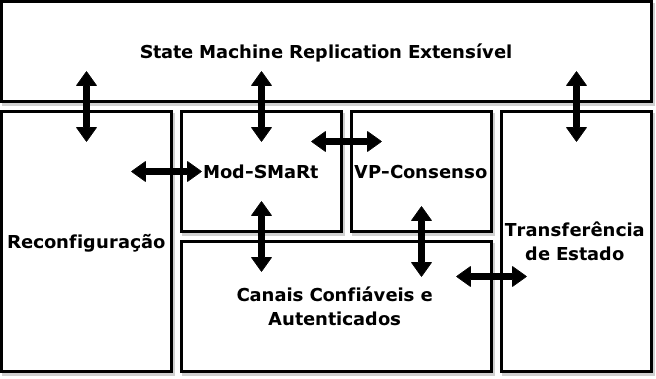
\includegraphics[clip,width=13.0cm]{images/image4.png}
				\caption{A modularidade do BFT-SMaRt. Adaptado de Alchieri~\cite{bessani3}}
				\label{fig:vis_sis}
			\end{center}
		\end{figure}
		
		%\item  Interface de Programação de Aplicação Simples e Extensível\\
		\subsection{Interface de Programação de Aplicação Simples e Extensível}
		A biblioteca java encapsula toda a complexidade de uma replicação de máquinas de estado tolerante a falhas bizantinas (BFT SMR) dentro de uma API que pode ser utilizada para a implementação de serviços determinísticos. Utilizando métodos \textit{invoke}(comando) para enviar comandos às réplicas que implementam o método \textit{execute}(comando) cujo objetivo é processar o comando recebido. Entretanto, caso a aplicação necessite de comportamentos especializados não suportado por este modelo de programação é possível utilizar outras chamadas ou \textit{plug-ins} tanto no lado do cliente quanto do servidor.\\
		
		
		%\item Consciência de ambiente Multi-Core\\
		\subsection{Percepção de ambiente Multi-Core}
		\textit{BFT-SMaRt} é capaz de aproveitar a arquitetura \textit{multicore} dos servidores para diminuir o tempo de processamento em regiões críticas do protocolo.\\
		
		%\item Modelo do Sistema\\
		\subsection{Modelo do Sistema}
		\textit{BFT-SMaRt} assume o modelo usual para sistemas BFT SMR: são necessárias n $\geq$ 3f+1 réplicas para tolerar f falhas bizantinas. Entretanto, visto que o sistema suporta reconfiguração, é possível modificar n e f em tempo de execução. Além disso, o sistema permite ser configurado para utilizar apenas n $\geq$ 2f+1 réplicas para tolerar f falhas de sistema. Porém, independente da configuração, o sistema necessita de conexões ponto-a-ponto confiáveis entre os processos de comunicação. Essa conexão é realizada utilizando \textit{message authentication code} (MAC) sobre o protocolo TCP/IP.\\
	%\end{itemize}
	
	\section{Protocolos Centrais}
	
	%\begin{itemize}
		%\item Total Order Multicast\\
		\subsection{\textit{Total Order Multicast}}
		Em um sistema distribuído, um algoritmo de ordenamento total é um protocolo de mensagem \textit{broadcast} que garante a entrega das mensagens de forma confiável e na mesma ordem para todos os participantes.\\
		
		O ordenamento total \textit{multicast} é possível graças ao \textit{Mod-SMaRt}, um protocolo modular que implementa BFT SMR utilizando uma primitiva de consenso. Durante sua fase de execução normal, a qual ocorre na ausência de falhas e na presença de sincronismo entre as outras réplicas, clientes enviam suas solicitações para todas as réplicas e aguardam pela resposta. O ordenamento total é alcançado através de uma sequência de instâncias de consenso, cada uma delas decidindo sobre um lote de solicitações de clientes. Cada instância é composta por três passos de comunicação. O primeiro passo solicita que o líder do consenso envie uma mensagem de \textit{PROPOSE} para cada réplica. Esta etapa é seguida por duas etapas de mensagens de todos para todos compostas de mensagens \textit{WRITE} e \textit{ACCEPT}. Onde as mensagens de \textit{PROPOSE} contém o lote de solicitações, \textit{WRITE} e \textit{ACCEPT} contém o \textit{hash} criptografado do lote.\\
		
		Quando uma falha ocorre ou alguma replica encontra-se dessincronizada das demais, o \textit{Mod-SMaRt} pode mudar para a fase de sincronização. Durante esta fase um novo líder é eleito e as réplicas são forçadas a entrarem na mesma instância de consenso. Este “pulo” pode causar com que algumas réplicas ativem o protocolo de transferência de estados.\\
		
		%\item Transferência de Estado\\
		\subsection{Transferência de Estado}
		A fim de implementar uma SMR que possa ser usada na prática, faz-se necessário que as réplicas possam ser reparadas e reintegradas ao sistema sem que todo o sistema de replicação seja reiniciado. Para garantir tal característica, o \textit{BFT-SMaRt} implementa algumas ideias chaves: (1) armazenar o log dos lotes de operações em execução em apenas um disco, (2) tirar instantâneos de estados (\textit{snapshots}) em diferentes pontos da execução em várias réplicas e (3) realizar transferência de estados de forma colaborativa, cada réplica enviando diferentes partes do estado para a réplica que está sendo recuperada.\\
	%\end{itemize}
	
	\section{Reconfiguração}
	O \textit{BFT-SMaRt} provê um protocolo especial que permite a adição ou execução de réplicas em tempo de execução. Porém, tal processo só pode ser iniciado pelos administradores executando um cliente com permissão de gerenciamento (\textit{View Manager}), por motivos de segurança.\\
	
	\section{Implementação}
	\textit{BFT-SMaRt} foi desenvolvido contendo menos de treze mil e quinhentas linhas de código Java distribuídos em cerca de noventa arquivos. Tal característica é significativamente menor do que ocorre em sistemas similares que geralmente possuem mais de vinte mil linhas de código. \\
	
	Um ponto chave quando se está implementando um mediador (\textit{middleware}) de replicação de alta vazão é como separar as várias tarefas do protocolo em uma arquitetura eficiente e robusta. No caso de uma replicação de máquinas de estado tolerante a falhas bizantinas (BFT SMR) existem dois requisitos adicionais: o sistema precisa lidar com centenas de clientes e resistir a possíveis comportamentos maliciosos tanto por parte dos clientes quantos das outras replicas.\\
	
	A Figura \ref{fig:image5} apresenta a arquitetura central com as \textit{threads}  usadas para o processamento das mensagens arquitetadas pela implementação do protocolo. Nesta arquitetura, todas as \textit{threads} comunicam através de filas delimitadas. A figura também mostra qual \textit{thread} alimenta e consume informações de cada fila. \\  
	
	\begin{figure}[htb]
		\begin{center}
			
			\includegraphics[clip,scale=0.57]{images/image5.png}
			\caption{Processamento de mensagens arquitetadas entre replicas do \textit{BFT-SMaRt}. Adaptado de Alchieri~\cite{bessani3} }
			\label{fig:image5}
		\end{center}
	\end{figure}
	
	As solicitações dos clientes são recebidas através do estoque de \textit{thread} provida pelo \textit{Framework} de comunicação \textit{Netty}. Assim que uma mensagem proveniente do cliente é recebida, é verificado se trata-se de uma solicitação ordenada ou não ordenada. Solicitações não ordenadas, as quais são geralmente aplicadas por comandos de apenas leitura, são entregadas diretamente para o serviço de implementação. No caso de uma solicitação ordenada, elas são entregues para o gerenciador de clientes, o qual verifica a integridade da solicitação, caso esteja integra, a solicitação é encaminhada para a fila do respectivo cliente. Perceba que o endereço MAC dos clientes são verificados pelo \textit{Netty threads}, desta forma as máquinas \textit{multi-core} e multi-processadas vão naturalmente aproveitar de seu poder para conquistar uma alta vazão. \\ 
	
	A \textit{thread} proponente é responsável por juntar uma carga de solicitações e transmitir a mensagem \textit{PROPOSE} do protocolo de consenso. O BFT-SMaRt preenche carga com solicitações pendentes até que: (a) seu tamanho alcance o máximo definido no arquivo de configuração; ou (b) não haja mais solicitações sobrando para serem adicionadas. Esta \textit{thread} só está ativa na replica líder. \\
	
	Cada mensagem \textit{m} que deve ser enviada de uma réplica para outra é colocada na fila de saída pela qual uma \textit{thread} emissora vai serializar a mensagem \textit{m}, produzir o endereço MAC que será anexado na mensagem e, enfim, enviar utilizando \textit{sockets TCP}. Do ponto de vista da réplica que irá receber a mensagem, uma \textit{thread} receptora vai ler \textit{m}, autenticar (validar seu MAC), desserializar e colocar na fila de entrada, onde todas as mensagens recebidas de outras réplicas são armazenadas em ordem para serem processadas.  \\
	
	A \textit{thread} processadora de mensagens é responsável por processar as mensagens provenientes do protocolo \textit{BFT SMR}. Esta \textit{thread} carrega as mensagens da fila de entrada e as processam caso façam parte do consenso que está sendo executado, entretanto, caso a mensagem pertença a um consenso que ainda será executado, ela é processada posteriormente, quando seu consenso estiver ativo. Caso a mensagem não se encaixe em nenhum dos dois cados, ela é apenas descartada. \\
	
	 Quando um consenso chega ao fim em uma réplica, ele é marcado como decidido e a carga que o possui também é marcada como decidida e colocada na fila das cargas decididas. Então, a \textit{thread} de entrega é chamada para coletar as cargas que estejam armazenados nesta fila, desserializar todas as solicitações da carga, remover cada uma delas das filas de seus respectivos clientes e marcar o  consenso corrente como finalizado. Após isso, a \textit{thread} de entrega invoca o serviço de réplica  para executar a solicitação e gerar a reposta correspondente. Quando terminar de gerar a resposta, o serviço de réplica a adiciona na fila de resposta. A \textit{thread} de resposta carrega as respostas armazenadas nessa fila e as manda para seus referidos clientes. \\
	 
	 O cronômetro de pedido da \textit{thread} é ativado periodicamente afim de verificar se alguma solicitação permanece como não respondida por mais tempo do que o delimitado por um tempo de \textit{timeout} predefinido em alguma fila de solicitações. A primeira vez que este cronômetro expira para alguma solicitação, faz com que ela seja encaminhada para o líder corrente. A segunda vez que este cronômetro expira para a mesma solicitação, a instância atual do protocolo de consenso é paralisado e a fase de sincronização é ativada. A base lógica destes cronômetros é a seguinte: dada uma rede em condições normais, o \textit{timeout} pode ser causado por algum cliente que não enviou a solicitação ao líder ou pelo líder que não encaminhou os pedidos das solicitações dos clientes. Visto que tipicamente existem muitos clientes para poucos servidores, é esperado que ocorra mais falhas no lado dos clientes do que dos servidores, por isto o protocolo do \textit{BFT-SMaRt} assume que o erro ocorreu no lado do cliente, suspeita-se do líder somente se o problema persistir. \\
	 
	 \section{Configurações Alternativas}
	 
	 Como mencionado nas seções anteriores, por padrão o \textit{BFT-SMaRt} tolera falhas bizantinas não maliciosas. Entretanto, o sistema pode ser configurado para suportar dois outros modelos de falhas.\\
	 
	 %\begin{itemize}
	 	%\item \textit{Crash Fault Tolerance} \\
	 	\subsection{Falhas de Sistema}
	 	\textit{BFT-SMaRt} suporta uma configuração de um parâmetro que caso seja ativado faz com que o sistema tolere apenas falhas de sistema. Quando esta propriedade está ativa, o sistema tolera  f \textless  n/2 (minoria simples), o que implica alterações em todos os passos necessários do protocolo, inclusive ignorando o passo de \textit{WRITE} durante a execução do consenso. Fora essas alterações, os protocolos são os mesmos do caso de tolerância de falha bizantina. 
	 	
	 	%\item Falhas Bizantinas Maliciosas\\
	 	\subsection{Falhas Bizantinas Maliciosas}
	 	Trabalhos anteriores ao \textit{BFT-SMaRt} demonstraram que o uso de assinaturas com chaves públicas sobre solicitações tornam impossível para os clientes forjarem vetores MAC e forçar que o líder seja alterado. Por padrão, o \textit{BFT-SMaRt} não utiliza assinaturas de chave pública além da utilizada para estabelecer chaves simétricas compartilhadas entre réplicas e durante a mudança do líder. Contudo, o sistema opcionalmente permite o uso de solicitações assinadas para evitar esse problema.\\
	 	
	 	Os mesmos trabalhos também mostram que líderes maliciosos podem lançar ataques de degradação de performance indetectáveis, fazendo com que a vazão do sistema caia drasticamente. Até o presente momento, o \textit{BFT-SMaRt} não apresenta meios de defesa contra este tipo de ataque. \\
	 	
	 	Por fim, o fato do \textit{BFT-SMaRt} ter sido desenvolvido em Java faz com que seja fácil aplicar o sistema em diferentes plataformas. Esta escolha permitiu que o time de desenvolvimento evitasse falhas de um único nó causadas por eventos acidentais (por exemplo, algum \textit{bug} ou problemas de infraestrutura) ou ataques maliciosos aproveitando de vulnerabilidades comuns.  \\
	 %\end{itemize}
	   
	
	%texto.... referência \cite{borsley96}
		
		\section{Conclusões do Capítulo}
	Neste capítulo foi detalhado a biblioteca \textit{BFT-SMaRt} apresentando seu conceito, princípios de projeto, protocolos centrais, reconfiguração, implementação e configurações alternativas.	Estes conceitos são fundamentais para a construção de um serviço de metadados possuindo alta confiabilidade e disponibilidade. 
	